% !TEX root = ../main.tex
\chapter{Employ the Learned Deep Model}\label{ch:chapter5} % For referencing the chapter elsewhere, use \ref{Chapter1}
%
%%----------------------------------------------------------------------------------------
%
After obtaining the learned models which exhibit desired behavior, 
their integration into the reference software is carried out.
In this chapter, the time cost of the model prediction
is analyzed and optimizing methods are described.
After that we explain the details of the algorithm for integration.
In the end of the chapter the results of experiments 
are presented with discussions.

%3D Video applications are attracting more interests
%%----------------------------------------------------------------------------------------
%
\section{Analysis and Optimisation for Prediction Time}\label{sec:analysis-and-optimization}
% In C++ APIs from Tensorflow version 1.1, if we want to run the prediction,
% a unique session has to be initialized in which the predicting activities 
% take place.
% It is found that the session initialization is very time expensive.
It is intuitive to think in this way: 
every time when the encoder encounters a new block in the video frames,
the learned models are required to perform the prediction for that block.
However, after this idea has been implemented, it turns out the
time cost of the encoder with neural engine even gets much higher 
than the encoder without neural engine.
We found that the idea of one prediction for one block actually
introduces a problem that impedes the integration to work as expected:
a new session is initialized for a prediction, and the initialization
for a single session in Tensorflow C++ APIs actually is very time
expensive.
The other idea which is a better way would be a single 
session for a batch of blocks.

The time cost of session initialization has been investigated
and compared between the two ideas aforementioned.
The learned model for blocks of size \(8\times8\) is loaded 
to run predictions for blocks of size \(8\times8\) from one single
frame in one video sequence with the resolution to 
be \(1024\times768\).
Totally 12288 blocks to predict.
When compiling the executable binary of the encoder
powered by neural engine, it can be compiled 
against CPU or GPU when the compilation tool 
called Bazel~\parencite{RN200} is utilized.
Even more, with Bazel, the AVX and SSE4.2 can be employed to
accelerate the parallel computations in one instruction
at single moment in CPU\@.
They offer more efficient matrix computations
to CPU\@.
Six experiments have been conducted and the results
are shown in 
Table~\ref{tab:seesion-init-plain-cpu}.
% on page~\pageref{tab:seesion-init-plain-cpu}.

\begin{table}
    \caption{Time cost of session initialization for two ideas based on three sets of compiling configurations}
    \bigskip\label{tab:seesion-init-plain-cpu}
    \centering
    \begin{tabular}{c c c c c}
        \toprule
        \# & Idea & Plain CPU & AVX and SSE4.2 & AVX, SSE4.2 and GPU \\
        \midrule
        1 & initialize 1 session for 12288 blocks & 21.37s &15.56s&2.03s \\
        2 & initialize 12288 sessions for 12288 blocks & 47.81s &33.91s&55.26s\\
        \bottomrule
    \end{tabular}
\end{table}

Obviously the best way is to compile the 
executable binary against AVX, SSE4.2 and GPU, at the same
time use the idea of one session for multiple blocks.

\section{The Integration of the Learned Model}\label{sec:integration-of-learned-model}
\begin{figure}
    \centering
    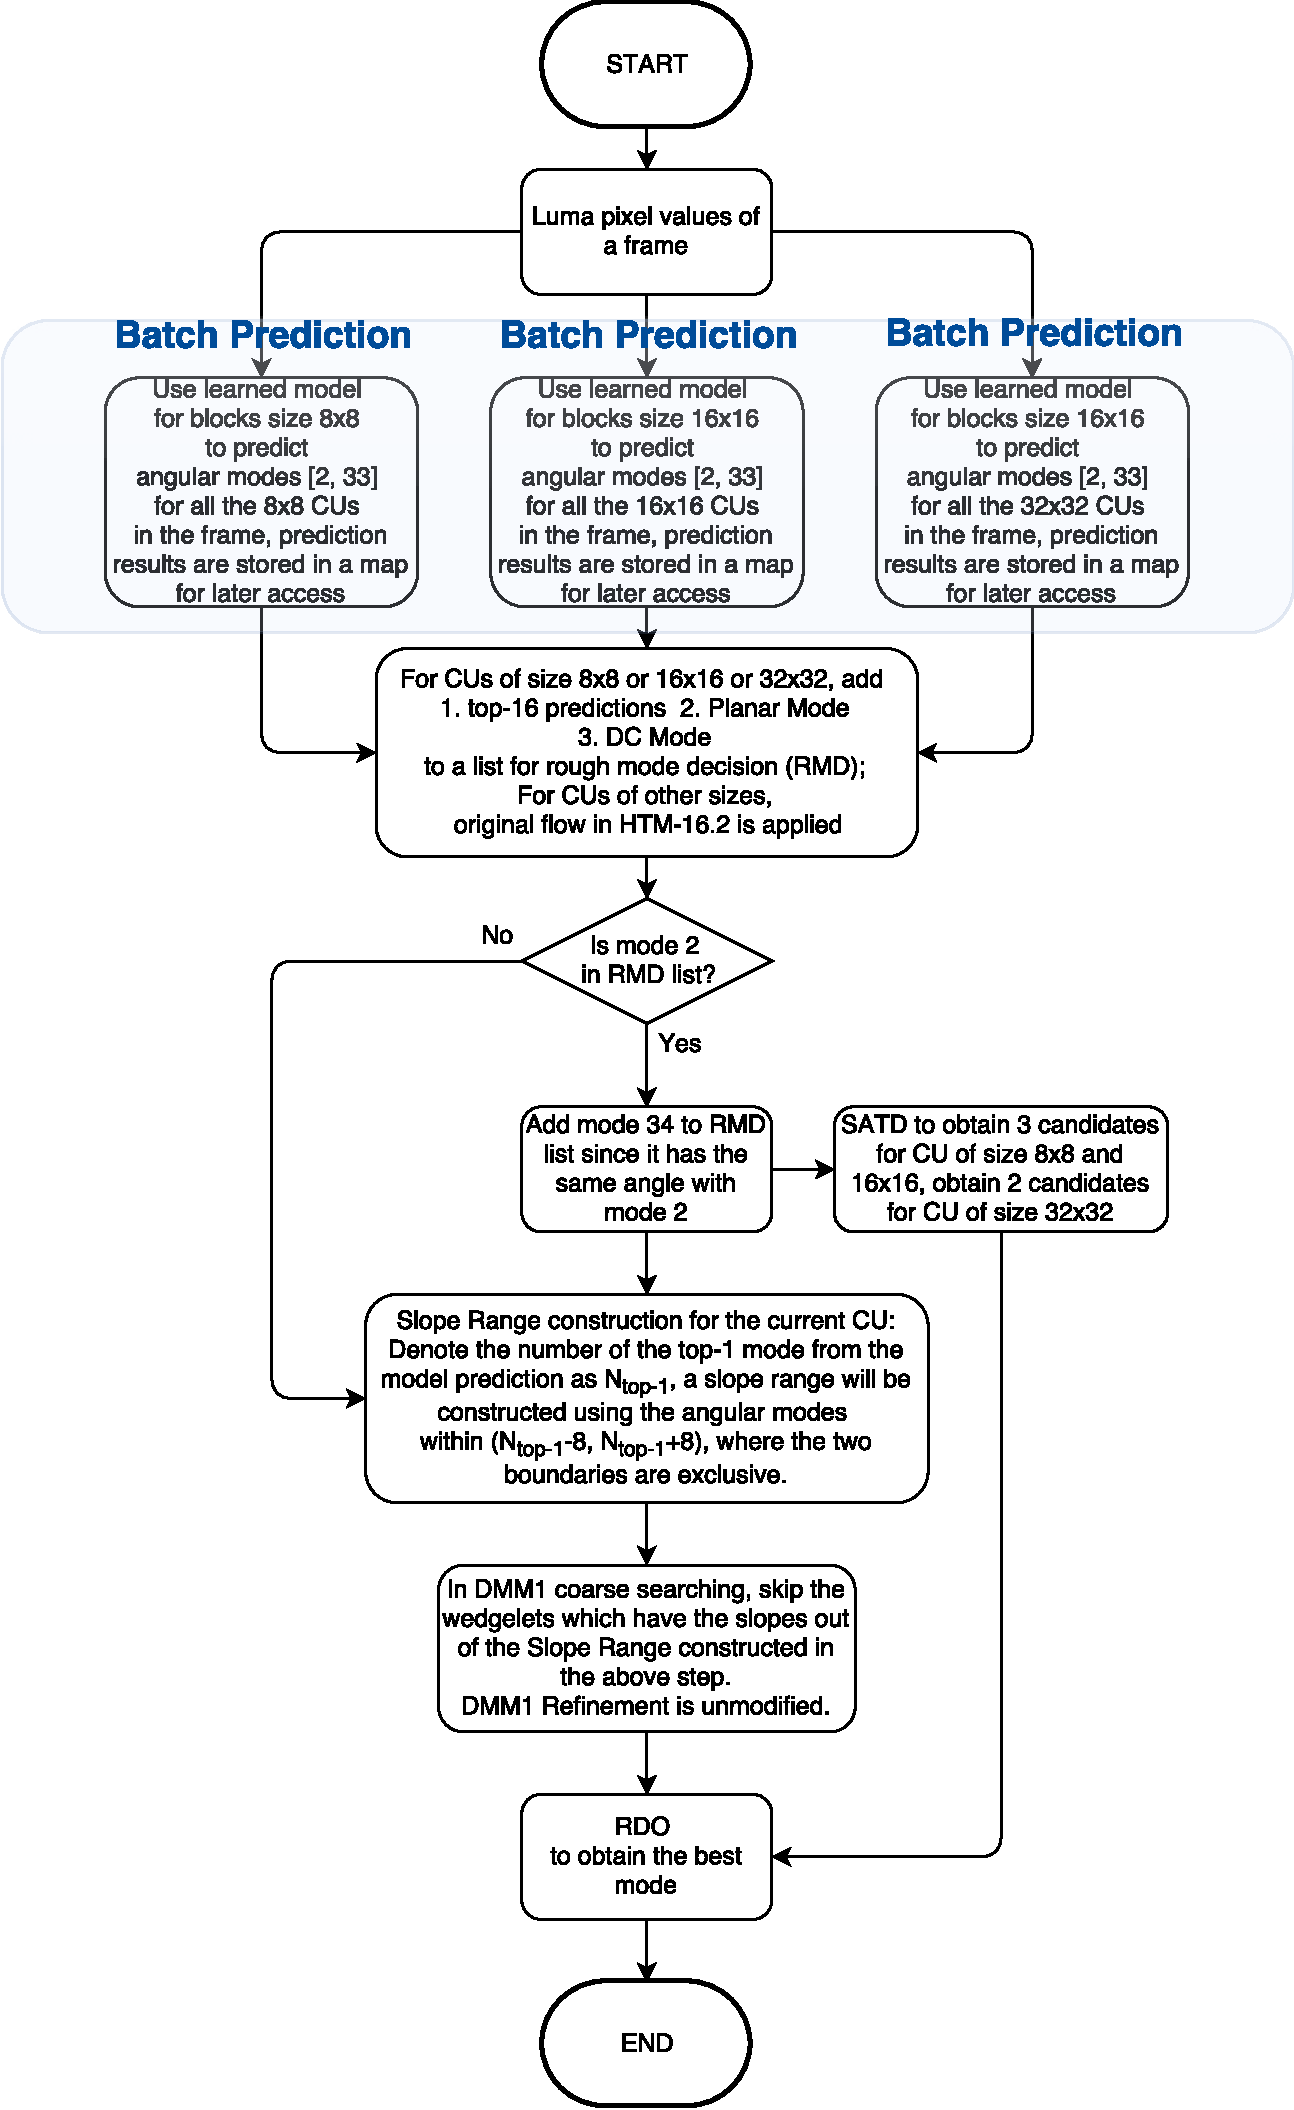
\includegraphics[width=\textwidth,height=\textheight,keepaspectratio]{Figures/proposed-fast-depth-coding-algorithm}
    \caption[Flowchart for proposed fast depth coding 
    algorithm]{Flowchart for proposed fast depth coding 
    algorithm.}\label{fig:proposed-fast-depth-coding-algorithm}
\end{figure}
\section{Results of Experiments}\label{sec:simu-results}
\section{Discussion}\label{sec:simu-discussion}

%Welcome to this \LaTeX{} Thesis Template, a beautiful and easy to use template for writing a thesis using the \LaTeX{} typesetting system.
%
%If you are writing a thesis (or will be in the future) and its subject is technical or mathematical (though it doesn't have to be), then creating it in \LaTeX{} is highly recommended as a way to make sure you can just get down to the essential writing without having to worry over formatting or wasting time arguing with your word processor.
%
%\LaTeX{} is easily able to~\parencite{RN93} professionally typeset documents that run to hundreds or thousands of pages long. With simple mark-up commands, it automatically sets out the table of contents, margins, page headers and footers and keeps the formatting consistent and beautiful. One of its main strengths is the way it can easily typeset mathematics, even \emph{heavy} mathematics. Even if those equations are the most horribly twisted and most difficult mathematical problems that can only be solved on a super-computer, you can at least count on \LaTeX{} to make them look stunning.
%
%%----------------------------------------------------------------------------------------
%
%\section{Welcome and Thanku}\label{sec:welome}
%Welcome to this \LaTeX{} Thesis Template, a beautiful and easy to use template for writing a thesis using the \LaTeX{} typesetting system.
%
%If you are writing a thesis (or will be in the future) and its subject is technical or mathematical (though it doesn't have to be), then creating it in \LaTeX{} is highly recommended as a way to make sure you can just get down to the essential writing without having to worry over formatting or wasting time arguing with your word processor.
%
%\LaTeX{} is easily able to professionally typeset documents that run to hundreds or thousands of pages long. With simple mark-up commands, it automatically sets out the table of contents, margins, page headers and footers and keeps the formatting consistent and beautiful. One of its main strengths is the way it can easily typeset mathematics, even \emph{heavy} mathematics. Even if those equations are the most horribly twisted and most difficult mathematical problems that can only be solved on a super-computer, you can at least count on \LaTeX{} to make them look stunning.
%
%%----------------------------------------------------------------------------------------
%
%\section{Welcome and ThYou}\label{sec:weome}
%Welcome to this \LaTeX{} Thesis Template~\parencite{Reference1}, a beautiful and easy to use template for writing a thesis using the \LaTeX{} typesetting system.
%
%If you are writing a thesis (or will be in the future) and its subject is technical or mathematical (though it doesn't have to be), then creating it in \LaTeX{} is highly recommended as a way to make sure you can just get down to the essential writing without having to worry over formatting or wasting time arguing with your word processor.
%
%\LaTeX{} is easily able to professionally typeset documents that run to hundreds or thousands of pages long. With simple mark-up commands, it automatically sets out the table of contents, margins, page headers and footers and keeps the formatting consistent and beautiful. One of its main strengths is the way it can easily typeset mathematics, even \emph{heavy} mathematics. Even if those equations are the most horribly twisted and most difficult mathematical problems that can only be solved on a super-computer, you can at least count on \LaTeX{} to make them look stunning.
%
%%----------------------------------------------------------------------------------------
%
%\section{Welcome and Thau}\label{sec:welcoe}
%Welcome to this \LaTeX{} Thesis Template, a beautiful and easy to use template for writing a thesis using the \LaTeX{} typesetting system.
%
%If you are
%\begin{table}
%
%    \label{tab:treatments}
%    \centering
%%    \begin{tabular}{l l l}
%%        \toprule
%%        \tabhead{Groups} & \tabhead{Treatment X} & \tabhead{Treatment Y} \\
%%        \midrule
%%        1 & 0.2 & 0.8\\
%%        2 & 0.17 & 0.7\\
%%        3 & 0.24 & 0.75\\
%%        4 & 0.68 & 0.3\\
%%        \bottomrule\\
%%    \end{tabular}
%    \begin{tabular}{c r @{.} l}
%        Pi expression       &
%        \multicolumn{2}{c}{Value} \\
%        \hline
%        $\pi$               & 3&1416  \\
%        $\pi^{\pi}$         & 36&46   \\
%        $(\pi^{\pi})^{\pi}$ & 80662&7 \\
%    \end{tabular}
%    \caption{The effects of treatments X and Y on the four groups studied.}
%\end{table}
%writing a thesis (or will be in the future) and its subject is technical or mathematical (though it doesn't have to be), then creating it in \LaTeX{} is highly recommended as a way to make sure you can just get down to the essential writing without having to worry over formatting or wasting time arguing with your word processor.
%
%\LaTeX{} is easily able to professionally typeset documents that run to hundreds or thousands of pages long. With simple mark-up commands, it automatically sets out the table of contents, margins, page headers and footers and keeps the formatting consistent and beautiful. One of its main strengths is the way it can easily typeset mathematics, even \emph{heavy} mathematics. Even if those equations are the most horribly twisted and most difficult mathematical problems that can only be solved on a super-computer, you can at least count on \LaTeX{} to make them look stunning.
%
%%----------------------------------------------------------------------------------------
%
%\section{Welcome and Tnk You}\label{sec:wlcome}
%Welcome to this \LaTeX{} Thesis Template, a beautiful and easy to use template for writing a thesis using the \LaTeX{} typesetting system.
%
%If you are writing a thesis.
%
%%\begin{verbatim}
%\begin{figure}
%    \centering
%    
\includegraphics{Figures/Electron}
%    %    \decoRule
%    \caption[An Electron]{An electron (artist's impression).}
%    \label{fig:Electron}
%\end{figure}
%%\end{verbatim}
%(or will be in the future) and its subject is technical or mathematical (though it doesn't have to be), then creating it in \LaTeX{} is highly recommended as a way to make sure you can just get down to the essential writing without having to worry over formatting or wasting time arguing with your word processor.
%
%\LaTeX{} is easily able to professionally typeset documents that run to hundreds or thousands of pages long. With simple mark-up commands, it automatically sets out the table of contents, margins, page headers and footers and keeps the formatting consistent and beautiful. One of its main strengths is the way it can easily typeset mathematics, even \emph{heavy} mathematics. Even if those equations are the most horribly twisted and most difficult mathematical problems that can only be solved on a super-computer, you can at least count on \LaTeX{} to make them look stunning.
%
%%----------------------------------------------------------------------------------------